%==============================================================================
%== template for LATEX poster =================================================
%==============================================================================
%
%--A0 beamer slide-------------------------------------------------------------
\documentclass[final]{beamer}
\usepackage[orientation=portrait,size=a0,
            scale=1.25         % font scale factor
           ]{beamerposter}
           
\geometry{
  hmargin=2.5cm, % little modification of margins
}

%
\usepackage[utf8]{inputenc}
\usepackage{qrcode}  % Generate QR codes in LaTeX
\usepackage{array}

\linespread{1.15}
%
%==The poster style============================================================
\usetheme{sharelatex}

%==Title, date and authors of the poster=======================================
\title
[International Workshop On Integrated Nonlinear Microwave and Millimetre-wave Circuits, 5-6 July 2018, Brive-la-Gaillarde, France] % Conference
{ % Poster title
Multiport conversions between S, Z, Y, h, ABCD, and T parameters
}

\author{Tibault Reveyrand}
\institute[XLIM]{XLIM-UMR CNRS 7252, France}
\date{\today}



\begin{document}
\begin{frame}[t]
%==============================================================================
\begin{multicols}{3}
%==============================================================================
%==The poster content==========================================================
%==============================================================================

\section{Introduction}

This poster presents generalized formulation for conversions between electrical parameters matrices. The calculations for two-port devices, presented in ~\cite{Frickey1994}, are here extended for multiport systems.

\section{Definitions}
\structure{Submatrices partitioning:} 
The multiport approach consists on considering the S-parameters matrix of the device of interest as a partition of 4 submatrices. Ports are divided in 2 groups: external and internal ports. This kind of partitioning, illustrated here on a S matrix can be applied to Z, Y, h, ABCD and T matrices as well.


\vskip1ex
\begin{figure}
\centering
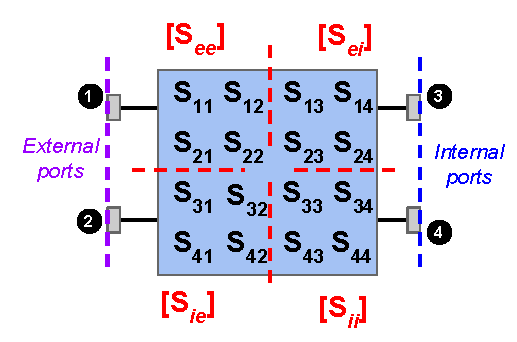
\includegraphics[width=0.55\columnwidth]{01_S4P_example}
\caption{Example of partitioning on a balanced multiport.}
\end{figure}
\vskip2ex
\structure{Electrical parameters:} 
Matrices defined in \cite{Frickey1994} can be expanded to multiport as follow:
\begin{equation*}
\begin{pmatrix}
   (V_e)\\
   (V_i) 
\end{pmatrix}
=\begin{bmatrix}
   [Z_{ee}]       & [Z_{ei}] \\
   [Z_{ie}]      & [Z_{ii}] 
\end{bmatrix}.
\begin{pmatrix}
   (I_e) \\
   (I_i) 
\end{pmatrix}
\label{def:Z}
\end{equation*}

\begin{equation*}
\begin{pmatrix}
   (I_e)\\
   (I_i) 
\end{pmatrix}
=\begin{bmatrix}
   [Y_{ee}]       & [Y_{ei}] \\
   [Y_{ie}]      & [Y_{ii}] 
\end{bmatrix}.
\begin{pmatrix}
   (V_e) \\
   (V_i) 
\end{pmatrix}
\label{def:Y}
\end{equation*}

\begin{equation*}
\begin{pmatrix}
   (V_e)\\
   (I_i) 
\end{pmatrix}
=\begin{bmatrix}
   [h_{ee}]       & [h_{ei}] \\
   [h_{ie}]      & [h_{ii}] 
\end{bmatrix}.
\begin{pmatrix}
   (I_e) \\
   (V_i) 
\end{pmatrix}
\label{def:h}
\end{equation*}

\begin{equation*}
\begin{pmatrix}
   (V_e)\\
   (I_e) 
\end{pmatrix}
=\begin{bmatrix}
   [A]       & [B] \\
   [C]      & [D] 
\end{bmatrix}.
\begin{pmatrix}
   (V_i) \\
   (-I_i) 
\end{pmatrix}
\label{def:ABCD}
\end{equation*}

\vspace{1cm}


\begin{equation*}
\begin{pmatrix}
   (b_e)\\
   (b_i) 
\end{pmatrix}
=\begin{bmatrix}
   [S_{ee}]       & [S_{ei}] \\
   [S_{ie}]      & [S_{ii}] 
\end{bmatrix}.
\begin{pmatrix}
   (a_e) \\
   (a_i) 
\end{pmatrix}
\label{def:S}
\end{equation*}


\begin{equation*}
\begin{pmatrix}
   (a_e)\\
   (b_e) 
\end{pmatrix}
=\begin{bmatrix}
   [T_{ee}]       & [T_{ei}] \\
   [T_{ie}]      & [T_{ii}] 
\end{bmatrix}.
\begin{pmatrix}
   (b_i) \\
   (a_i) 
\end{pmatrix}
\label{def:T}
\end{equation*}


Conversions can be calculated according to the power-waves definition by K. Kurokawa~\cite{Kurokawa1965}:

\begin{equation*}
\left\{
\begin{array}{rl}
  a_n &= \frac{1}{2.\sqrt{|\Re\{Z_n\}|}}.(V_n+Z_n.I_n) \\
  b_n &= \frac{1}{2.\sqrt{|\Re\{Z_n\}|}}.(V_n-Z^*_n.I_n)
\end{array}
\right.
\label{eq:kurokawa}
\end{equation*}
where $a_n$, $b_n$ and $Z_n$ are incident, reflected power waves, and reference impedance at port $n$ respectively.
\vskip2ex


\section{Matrices Conversions}
\structure{Electrical parameters matrices:} 
\begin{equation*}
[Y]={[Z]}^{-1}
\label{ZtoY}
\end{equation*}
\vspace{0.5cm}
\begin{equation*}
[Z]=
\begin{bmatrix}
   [A].{[C]}^{-1}       & [A].{[C]}^{-1}.[D]-[B] \\
   {[C]}^{-1}      & {[C]}^{-1}.[D]  
\end{bmatrix}
\end{equation*}

\begin{equation*}
\begin{bmatrix}
A & B \\ C & D
\end{bmatrix}=
\begin{bmatrix}
   \resizebox{0.21\hsize}{!}{$[Z_{ee}].{[Z_{ie}]}^{-1}$}       & \resizebox{0.4\hsize}{!}{$[Z_{ee}].{[Z_{ie}]}^{-1}.[Z_{ii}]-[Z_{ei}]$} \\
   \resizebox{0.11\hsize}{!}{${[Z_{ie}]}^{-1}$}      & \resizebox{0.2\hsize}{!}{${[Z_{ie}]}^{-1}.[Z_{ii}]$}
\end{bmatrix}
\end{equation*}
\begin{equation*}
[h]=
\begin{bmatrix}
   [Z_{ee}]-[Z_{ei}].{[Z_{ii}]}^{-1}.[Z_{ie}]       & [Z_{ei}].{[Z_{ii}]}^{-1} \\
   -{[Z_{ii}]}^{-1}.[Z_{ie}]      & {[Z_{ii}]}^{-1} 
\end{bmatrix}
\end{equation*}
\begin{equation*}
[Z]=
\begin{bmatrix}
   [h_{ee}]-[h_{ei}].{[h_{ii}]}^{-1}.[h_{ie}]       & [h_{ei}].{[h_{ii}]}^{-1} \\
   -{[h_{ii}]}^{-1}.[h_{ie}]      & {[h_{ii}]}^{-1} 
\end{bmatrix}
\end{equation*}


\vspace{1cm}


\begin{equation*}
[Y]=
\begin{bmatrix}
   [D].{[B]}^{-1}       & [C]-[D].{[B]}^{-1}.[A] \\
   -{[B]}^{-1}      & {[B]}^{-1}.[A]  
\end{bmatrix}
\end{equation*}
\begin{equation*}
\begin{bmatrix}
A & B \\ C & D
\end{bmatrix}=
\begin{bmatrix}
   \resizebox{0.21\hsize}{!}{$-{[Y_{ie}]}^{-1}.[Y_{ii}]$}       & \resizebox{0.14\hsize}{!}{$-{[Y_{ie}]}^{-1}$} \\
   \resizebox{0.4\hsize}{!}{$[Y_{ei}]-[Y_{ee}].{[Y_{ie}]}^{-1}.[Y_{ii}]$}      & \resizebox{0.21\hsize}{!}{${-[Y_{ie}]}^{-1}.[Y_{ee}]$}
\end{bmatrix}
\end{equation*}
\begin{equation*}
[h]=
\begin{bmatrix}
   {[Y_{ee}]}^{-1}     & -{[Y_{ee}]}^{-1}.[Y_{ei}] \\
   [Y_{ie}].{[Y_{ee}]}^{-1}      & [Y_{ii}]-[Y_{ie}].{[Y_{ee}]}^{-1}.[Y_{ei}] 
\end{bmatrix}
\end{equation*}
\begin{equation*}
[Y]=
\begin{bmatrix}
   {[h_{ee}]}^{-1}       & -{[h_{ee}]}^{-1}.[h_{ei}] \\
   [h_{ie}].{[h_{ee}]}^{-1}     &  [h_{ii}]-[h_{ie}].{[h_{ee}]}^{-1}.[h_{ei}] 
\end{bmatrix}
\end{equation*}


\vspace{1cm}

\structure{Scattering parameters matrix [S]:}
\begin{equation*}
[Z]={[G_0]}^{-1}.{([I]-[S])}^{-1}.([S].[Z_0]+[Z^*_0]).[G_0]
\label{S2Z}
\end{equation*}
\begin{equation*}
[S]=[G_0].([Z]-[Z^*_0]).{([Z]+[Z_0])}^{-1}.[G_0]^{-1}
\label{Z2S}
\end{equation*}

\begin{equation*}
[Y]={[G_0]}^{-1}.{([S].[Z_0]+[Z^*_0])}^{-1}.{([I]-[S])}.[G_0]
\end{equation*}
\begin{equation*}
[S]=[G_0].([I]-[Z^*_0].[Y]).{([I]+[Z_0].[Y])}^{-1}.[G_0]^{-1}
\end{equation*}

with
\begin{equation*}
[G_0]=\text{diag} \{g_1,\dots,g_n,\dots, g_N\}
\label{G0}
\end{equation*}
\begin{equation*}
[Z_0] =\text{diag}\{Z_1,\dots,Z_n,\dots, Z_N\} 
\label{ref_impedance}
\end{equation*}
and $[I]$ is the identity matrix.
$[G_0]$ and $[Z_0]$ are diagonal matrices (terms outside the diagonal are zero) where each term is related to a port reference impedance $Z_n$ and
\begin{equation*}
g_n=\frac{1}{\sqrt{|\Re\{Z_n\}|}}
\end{equation*}


\vspace{1cm}
\structure{Transfert parameters matrix [T]:} 
\begin{equation*}
[T]=
\begin{bmatrix}
   {[S_{ie}]}^{-1}       & -{[S_{ie}]}^{-1}.[S_{ii}] \\
   [S_{ee}].{[S_{ie}]}^{-1}      & [S_{ei}]-[S_{ee}].{[S_{ie}]}^{-1}.[S_{ii}] 
\end{bmatrix}
\end{equation*}

\begin{equation*}
[S]=
\begin{bmatrix}
   [T_{ie}].{[T_{ee}]}^{-1} &  \;    & [T_{ii}]-[T_{ie}].{[T_{ee}]}^{-1}.[T_{ei}] \\
   {[T_{ee}]}^{-1}    & \;  & -{[T_{ee}]}^{-1}.T_{ei}
\end{bmatrix}
\end{equation*}
Chain matrices $[ABCD]$ and $[T]$ are properly defined only when the system is balanced (same number of internal and external ports). If the system is unbalanced, we have to ensure the uniqueness of the solution and then to apply the pseudo-inverse operator instead of the inverse matrix function.


 


\section{S-parameters Normalization}
The change of reference impedance of a multiport S-parameters $[S]$ matrix from $[Z_0]$ to $[Z'_0]$ is:
\begin{equation*}
[S']={[A]}^{-1}.([S]-[\rho^*]).{([I]-[\rho].[S])}^{-1}.[A^*]
\end{equation*}
where
\begin{equation*}
[A]={[G'_0]}^{-1}.[G_0].{\left[{[I]-[\rho^*]}\right]}^{-1}
\end{equation*}
\begin{equation*}
[\rho]={\left[{[Z'_0]-[Z_0]}\right]}.{\left[{[Z'_0]+[Z^*_0]}\right]}^{-1}
\end{equation*}
$[I]$ is the identity matrix, $[G_0]$, $[G'_0]$, $[Z_0]$ and $[Z'_0]$ are previously defined. All matrices, except $[S]$ and $[S']$, are diagonal matrices.

\section{Embedding}
The embedding procedure, and SnP reduction, consist on the S-parameters calculation at the external ports according to the perfectly known S-parameters connected at the internal ports. The formula is:
\begin{equation*}
[S_{Global}]=[S_{ee}]+[S_{ei}].{\left({[I]-[S_{L}].[S_{ii}]}\right)}^{-1}.[S_{L}].[S_{ie}]
\label{S_global}
\end{equation*}



%\vskip1ex
\begin{figure}
\centering
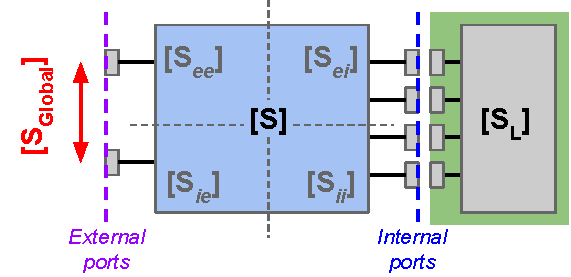
\includegraphics[width=0.55\columnwidth]{02_Embedding_SnP}
\caption{Illustration of an unbalanced multiport S-parameters terminated with a multiport load at its internals ports.}
\end{figure}
We can apply the same embedding procedure with $[Z]$ or $[Y]$ matrices without any condition on the multiport device:
\begin{equation*}
[Z_{Global}]=[Z_{ee}]-[Z_{ei}].{\left({[Z_{ii}]+[Z_{L}]}\right)}^{-1}.[Z_{ie}]
\end{equation*}
\begin{equation*}
[Y_{Global}]=[Y_{ee}]-[Y_{ei}].{\left({[Y_{ii}]+[Y_{L}]}\right)}^{-1}.[Y_{ie}]
\end{equation*}

%In all those equations, the matrix to invert is square. The embedding work whatever the system is balanced or not. Nevertheless, calculation of $[S_{Global}$ from $[T]$ only works  when the system is balanced, or when the number of internal port is higher than the external one ($[T]$ matrix transformation is lossy \cite{Frei2008}) as:
%\begin{equation*}
%[S_{Global}]=\left({[T_{ie}]+[T_{ii}].[S_{L}]}\right).{\left({[T_{ee}]+[T_{ei}].[S_{L}]}\right)}^{-1}
%\label{S_global}
%\end{equation*}

\section{De-embedding}
The de-embedding procedure consists on extracting the $[S_L]$ when $[S]$ and $S_{Global}$ are known:
\begin{equation*}
\begin{aligned}
%\begin{split}
\begin{bmatrix}
S_L
\end{bmatrix}
= &  {[S_{ei}]}^{-1}.([S_{Global}]-[S_{ee}])\\
       &.{\left[{[S_{ie}]+[S_{ii}].{[S_{ei}]}^{-1}.([S_{Global}]-[S_{ee}])}\right]}^{-1} 
%\end{split}
\end{aligned}
\label{de-emb}
\end{equation*}

The equation works only when $[S]$ describes a balanced system. If the number of internal ports ($N_i$) is lower than the number of external port ($N_e$), we can use the pseudo-inverse operator to invert $S_{ei}$ and get the least-square solution. Otherwise, the solution can not be solved and requires more assumptions. 


\vskip1ex
\begin{table}
\centering
%\caption{Illustration de-embedding witha  multiport. The first line represents a balanced system. The second line is an unbalanced system with a number of external ports higher than internal ones ($N_e > N_i$). The matrix inversion has to be done with the pseudo-inverse operator ($\bullet ^{+}$). The third line represents an unbalanced system where $N_i > N_e$. There is not uniqueness of the solution for the matrix inversion. }
\begin{tabular}{m{1cm} m{6cm} m{4cm} m{4cm} m{4cm}  }
\hline\hline
   & Test Fixture & \center $[S]$ & \center $[T]$ &  $[S_{L}]$ \\
\hline
   
\includegraphics[width=0.05\columnwidth]{Green.pdf} &  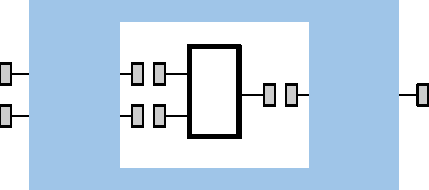
\includegraphics[width=0.20\columnwidth]{ST1.pdf} &  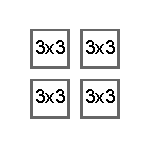
\includegraphics[width=0.20\columnwidth]{S1.pdf}   & 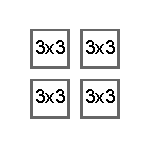
\includegraphics[width=0.20\columnwidth]{S1.pdf} &  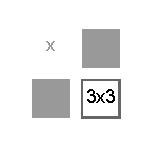
\includegraphics[width=0.20\columnwidth]{SD1.pdf}  \\
   
\includegraphics[width=0.05\columnwidth]{Green.pdf} & 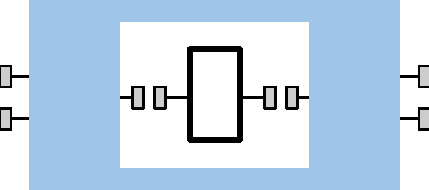
\includegraphics[width=0.20\columnwidth]{ST2.pdf}&  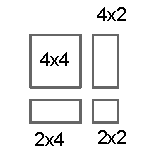
\includegraphics[width=0.20\columnwidth]{S2.pdf}   & 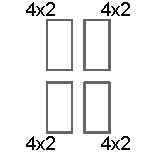
\includegraphics[width=0.20\columnwidth]{T2.pdf} & 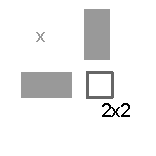
\includegraphics[width=0.20\columnwidth]{SD2.pdf} \\
   
\includegraphics[width=0.05\columnwidth]{Red.pdf} & 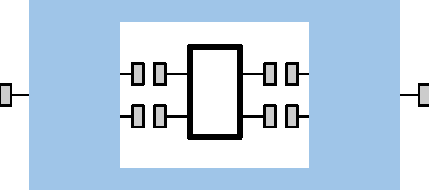
\includegraphics[width=0.20\columnwidth]{ST3.pdf} &  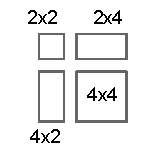
\includegraphics[width=0.20\columnwidth]{S3.pdf}   & 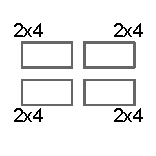
\includegraphics[width=0.20\columnwidth]{T3.pdf} & 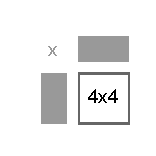
\includegraphics[width=0.20\columnwidth]{SD3.pdf} \\
   \hline\hline
\end{tabular}
\end{table}
\vskip2ex


This table illustrates a de-embedding on a multiport device. The first line represents a balanced system. The second line is an unbalanced system with $N_e > N_i$. The matrix inversion has to be done with the pseudo-inverse operator. The third line represents an unbalanced system with $N_i > N_e$. There is not uniqueness of the solution for the matrix inversion.
Note that S to T matrix transformation is lossy \cite{Frei2008} with unbalanced networks when $N_i > N_e$. 







\section{Conclusion}

This poster presents a multiport extension of the matrix parameters formulas by Frickey in 1994 \cite{Frickey1994}. The reader can handle, convert, normalize or reduce any matrix representing a linear multiport.



%==============================================================================
%==End of content==============================================================
%==============================================================================

%--References------------------------------------------------------------------

\subsection{References}

\bibliographystyle{IEEEtran}
\bibliography{IEEEabrv,biblio}

%\begin{thebibliography}{99}

%\bibitem{ref1} J.~Doe, Article name, \textit{Phys. Rev. Lett.}

%\bibitem{ref2} J.~Doe, J. Smith, Other article name, %\textit{Phys. Rev. Lett.}

%\bibitem{web} \url{http://www.google.pl}

%\end{thebibliography}
%--End of references-----------------------------------------------------------


% --- QRCODE
\subsection{Downloads}
\vskip1ex
\center 
\begin{tabular}{ccc}
   \qrcode[height=0.20\columnwidth]{http://www.microwave.fr/publications/151.pdf} & \hspace*{5cm} & \qrcode[height=0.20\columnwidth]{http://www.microwave.fr/publications/151p.pdf} \\
   PAPER & & POSTER \\
\end{tabular}




\end{multicols}

%==============================================================================
\end{frame}
\end{document}
